\documentclass[11pt]{article}
%this is for cyrillic text
\usepackage[main=russian,english]{babel}
%this is needed for changing font
\usepackage{fontspec}
\usepackage[a4paper, top=1cm]{geometry}
%without this double integral \iint doesnt work
\usepackage{mathtools}
\usepackage{physics}
%Чтобы LaTeX-овские лигатуры работали, типа тире, кавычек и прочего
\newfontfamily\cyrillicfont[Mapping=tex-text]{Times New Roman}
\usepackage{pgfplots}
\pgfplotsset{compat=1.8}
%this font has cyrillic letters
\setmainfont{Times New Roman}
\setlength{\parindent}{0pt}
\renewcommand{\labelenumi}{\Roman{enumi}}
\begin{document} 
\begin{center}
\begin{Large}
\textbf{Конспект по вычислительной математике} \\
\end{Large}
\end{center}
\[x_i = f(x_{i-1})\]
\[|x_i - x_{i-1}| < \varepsilon\]
\textbf{Решение трансцендентного уравнения} \\

Если на интервале $a, b$ функция $f(x)$ непрерывна и монотонна (имеет знакопостоянную производную), а её значения на концах интервала имеют разные знаки, то на рассматривоемом отрезке есть один и только один корень.

\begin{center}
 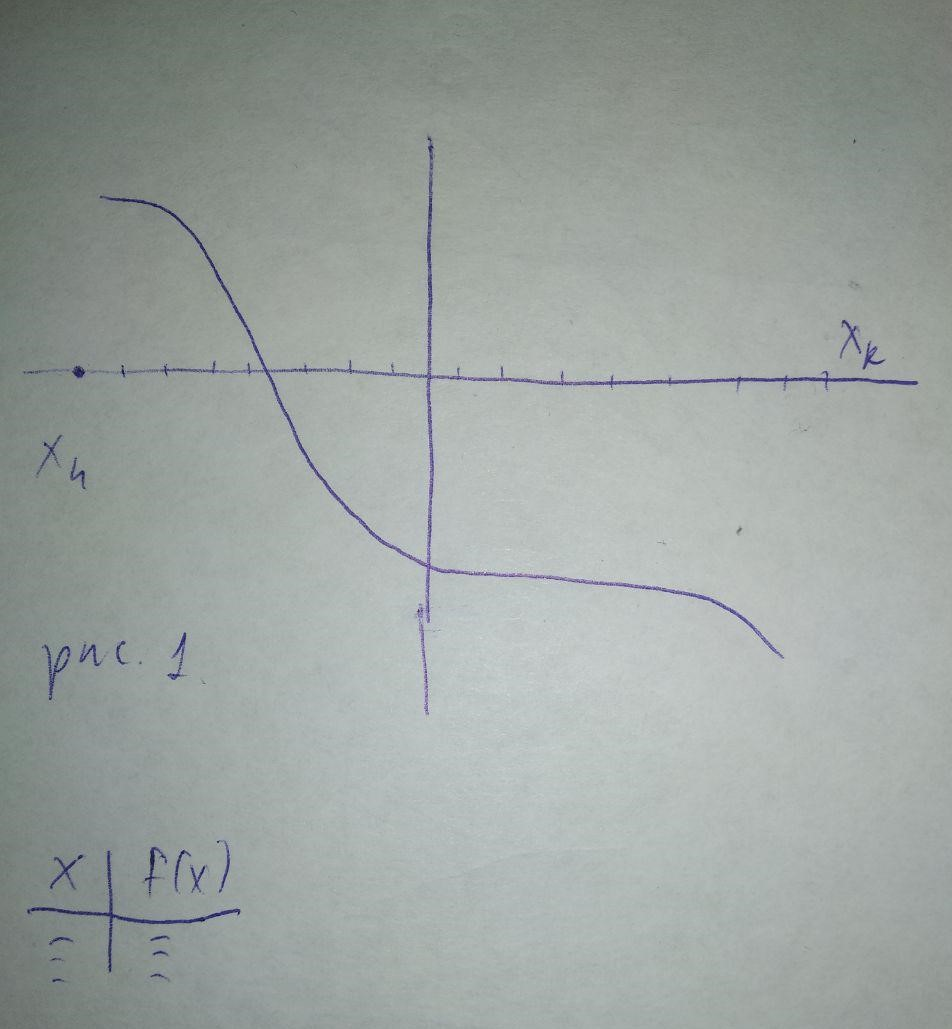
\includegraphics[scale=0.5]{рис1.jpg}
 \end{center} 

Решение сводится к нахождению интервала и уточнению по заданному методу. \\

{\large\textbf{Метод половинного деления}} \\
Находим середину отрезка

\begin{center}
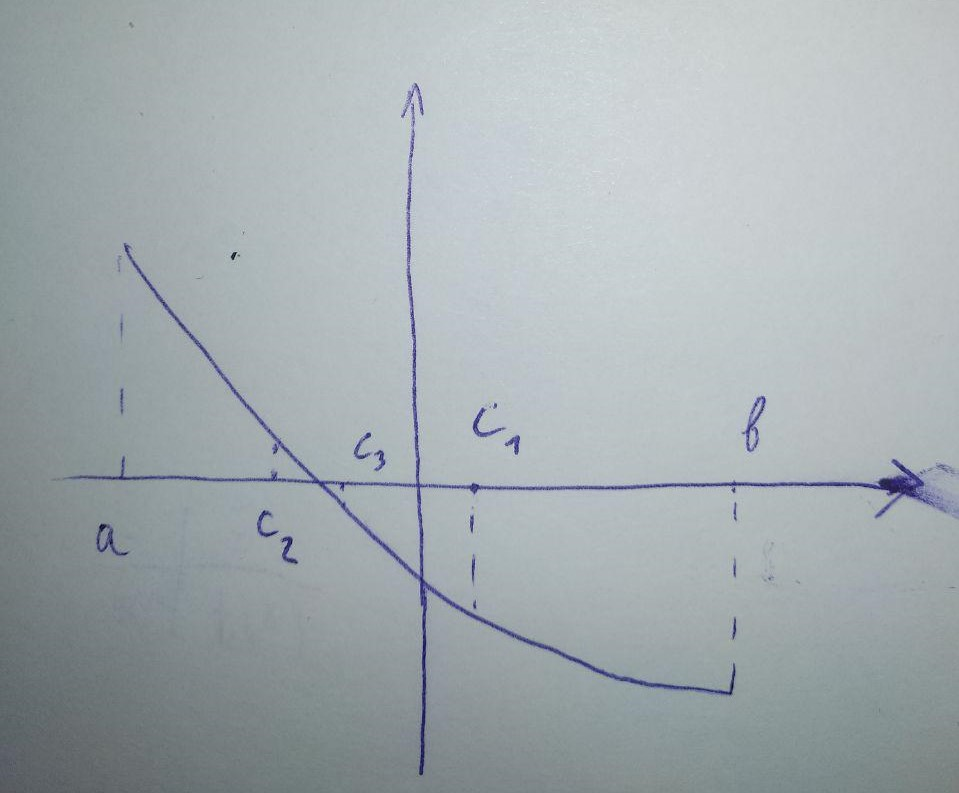
\includegraphics[scale=0.5]{рис2.jpg} 
\end{center}
 
Если $f(a) \cdot f(c) < 0$, то функция пересекает ось абсцисс на интервале $ac$, тогда в следующей итерации $a,c$ становится $ab$
 если $f(b) \cdot f(c) < 0$, то функция пересекает ось абсцисс на $bc$, $c \Rightarrow b = c$
 
 условие остановки $|a -b| < 2\varepsilon$ 

Метод применим даже к функциям с множеством перегибов и  с пересечениями оси абсцисс.
 
{\large \textbf{Метод хорд}}

\begin{center}
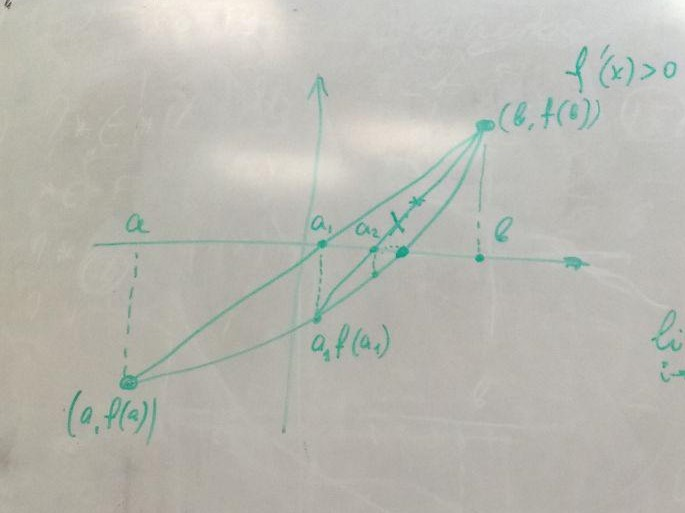
\includegraphics[scale=0.8]{рис3.jpg} 
\end{center}

Проводим хорду $ab$
\\
\[f'(x) > 0\]
\[\lim\limits_{i \to \infty}a_i = x^*\]

\[A(a_i f(a_i))\]
\[B (b, f(b))\]
\[\frac{I - f(a_i)}{f(b) - f(a_i)} = \frac{x-a}{b-a_i}\]
для $I = 0 \quad$ $x = a_{i+1}$

\[a_{i+1} = a_i - \frac{f(a_i)}{f(b) - f(a_i)}(b-a_i)\]

\begin{center}
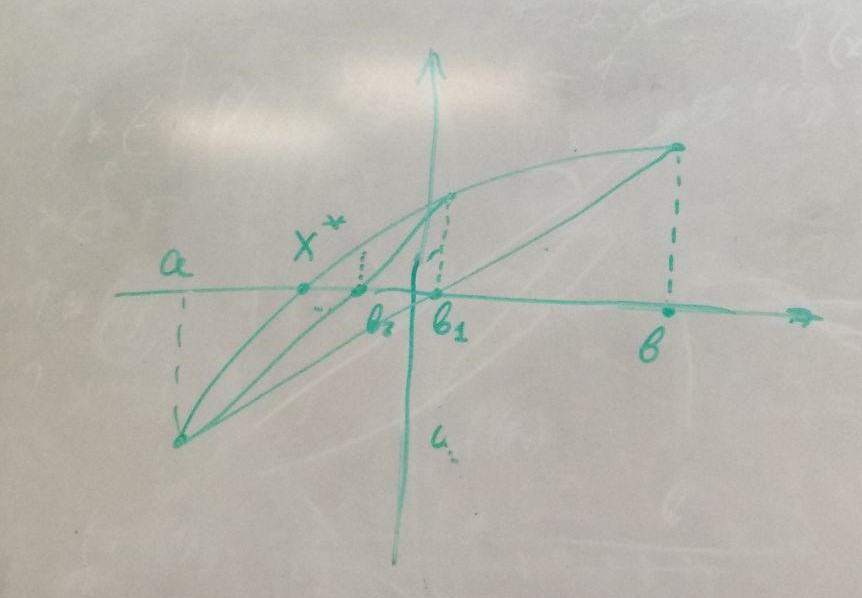
\includegraphics[scale=0.8]{рис4.jpg} 
\end{center}


\[b_{i+1} = b_i - \frac{f(b_i)}{f(b_i) - f(a)}(b_i - a)\]

В качестве неподвижного конца интервала рассматривается соотношение $f'(x) \cdot f''(x) > 0$, тот конец для которого оно выполняется , выбирается в качестве неподвижного.

Чтобы последовательность сходилась необходимо чтобы $f'(x) \quad \text{и} \quad f''(x) $ на всем интервале имели постоянный знак. 
Выбирается интервал, проверяется какой конец неподвижный и используется формула

Остановка когда \[|a_i - a_{i-1}| < \varepsilon\] \begin{center}
или
\end{center}
\[|b_i - b_{i-1}| < \varepsilon\]

\[Ch(x) = 1 + \frac{x^2}{2!} + \frac{x^4}{4!} + \cdots + \frac{x^{2n}}{(2n)!} + \cdots\]

Точность: \[\frac{x^{2n}}{(2n)!} < \varepsilon\]

\[\frac{x^{2n}}{(2n)!} \frac{(2(2n-1))!}{x^{2(n-1}} = \frac{x_i}{x_{i-1}} = D = \frac{x^{2}}{(2n-1)2n}\]
\end{document}